%%% Local Variables:
%%% mode: latex
%%% TeX-master: t
%%% End:

% !Mode:: "TeX:UTF-8"

\chapter{考虑温度对漏电流功耗影响的MPSoC结构级热分析算法}
\label{cha:SSTA}


\section{多核芯片热分析的研究对象建模}
\label{sec:SSTAbasic}

\subsection{芯片的散热系统}
图\ref{fig:cpu-disperse-package}给出了完整的芯片散热系统结构,在散热片下依次是导热层2(TIM2)、扩热层、导热层1(TIM1), 导热层1下方就是芯片的内核(die),注意:内核+导热层1+扩热层+散热片+风扇构成了芯片的主散热通道。 内核下方是芯片的封装基座,封装基座下方是芯片插座,芯片插座下方则是印刷电路版(PCB)。 需要特别指出:内核、封装基座、芯片插座和PCB构成了辅散热通道。散热通道的散热能力强于主散热通道辅近两三个数量级, 所以在各种规模各种粒度的芯片散热系统建模中,一般均只讨论主散热通道,而忽略辅散热通道。

\begin{figure}[H]
  \centering
  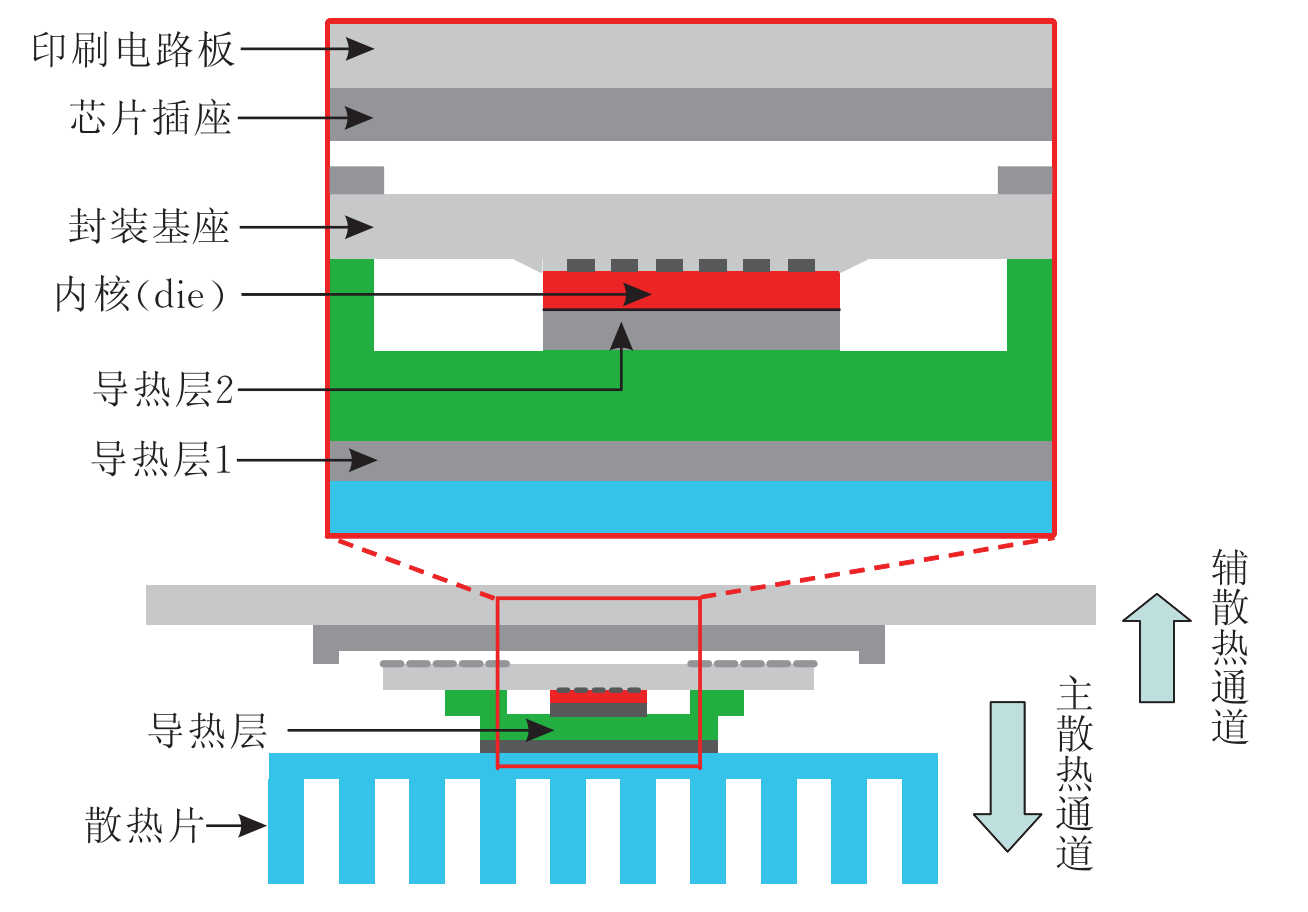
\includegraphics[width=0.7\textwidth,height=0.45\textheight]{CPUDispersePackage}
  \caption{IC散热系统的结构示意}
  \label{fig:cpu-disperse-package}
\end{figure}

从图\ref{fig:cpu-disperse-package}还可以看出,IC散热系统包括:内核的硅衬底、由硅胶或硅脂等软性材料构成的导热层、 由芯片金属壳构成的扩热层、及散热片等散热器件。 图\ref{fig:intel-fclg-package}为Intel公司FCLGA10的散热系统结构,可以看出, 在封装好的芯片内,芯片金属封盖起到扩热的作用;为了保护内核,封盖与内核之间采用的是一层很薄的软性材料(多数为硅脂)。

\begin{figure}[H]
  \centering
  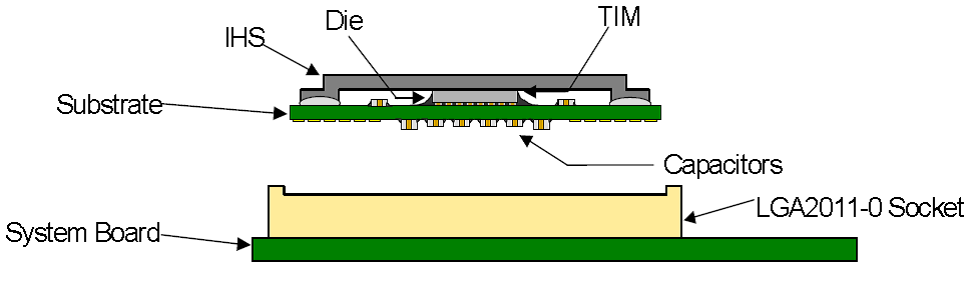
\includegraphics[width=0.9\textwidth,height=0.20\textheight]{IntelFCLG10Package}
  \caption{Intel公司FCLGA10封装的散热系统结构}
  \label{fig:intel-fclg-package}
\end{figure}

一般而言,芯片散热系统所用的导材料有:铜Cu(封盖与散热片)、硅Si(硅衬底)、硅胶或硅脂(导热层), 其中铜和硅的导热能力要远高于硅胶与硅脂。因此,在散热系统中,为了降低系统的热阻,必须尽量减小导热层的厚度, 但为了保证不损坏内核,金属封盖与内核之间的导热层厚度一般取0.5-0.8mm, 从图\ref{fig:intel-fclg-package}可以看出:Intel公司CPU芯片的导热层厚度要小于0.5mm,这主要取决于该公司的巨大技术实力。

\begin{table}
\centering
\caption{导热材料的热设计参数}
\begin{tabular}{c c c c}
\hline\hline
材料 & $k$($W/(cm \times K)$) & $\rho$($kg/cm^3$) & $c$($J/(kg \times K)$) \\ [0.5ex]
\hline
铜 & 4.00 & 0.00892 & 386.00  \\
硅 & 1.00 & 0.00232 & 171.00 \\
硅脂 & 0.04 & 0.00240 & NA \\
\hline
\end{tabular}
\label{tab:chap4:cu-si-material}
\end{table}

为了对芯片温度进行稳态或者瞬态分析,就必须对各传热器件进行热阻(热导)和热容的参数提取。 为此,我们将铜、硅、导热层(TIM)材料的热导率$k$(单位为$W/(cm \times K)$)、比重$\rho$ (单位为$kg/cm^3$)、比热容$c$(单位为$J/(kg \times K)$)列于表\ref{tab:chap4:cu-si-material}中。 对于作为导热层材料的硅脂,由于工艺不同,其参数变化较大,所以取上界。


\subsection{多核架构及其电热分布}

目前多核CPU普遍采用同质架构。即每个核心(core)拥有相同的逻辑功能模块(computing unit)、容量相同的专享缓存(exclusive cache),占有相同的内核面积, 同时共享最后一级缓存(last level cache,LLC)缓存、I/O等功能模块\onlinecite{TemMicroArch,TemMicArcMdlImpl}。 每个核心具有相同数量的工作模式,不同的工作模式意味着消耗不同程度的能量。一般来说,每个核心除具有一个全速高能模式外, 还具有多种耗能程度不同的节能模式\onlinecite{ThrOptTskAllocThemConstMulPro}。
在每个核心内,逻辑功能模块具有最大的功耗密度,该功能模块对应的指令L1缓存和数据L1缓存功耗密度次之, L2缓存具有的功耗密度相较而言最小。由于注入的热量大,每个核的热点(温度最高点)出现在逻辑功能模块,所以在物理设计中, 理论上说,要将逻辑功能模块布放在散热条件好的芯片边沿处,而散热条件最差的芯片中央布放功耗密度最小的LLC,从而降低芯片的热点温度。 图\ref{fig:ev6}为Alpha 21264芯片的物理布局\onlinecite{TemMicroArch},

\begin{figure}[H]
  \centering
  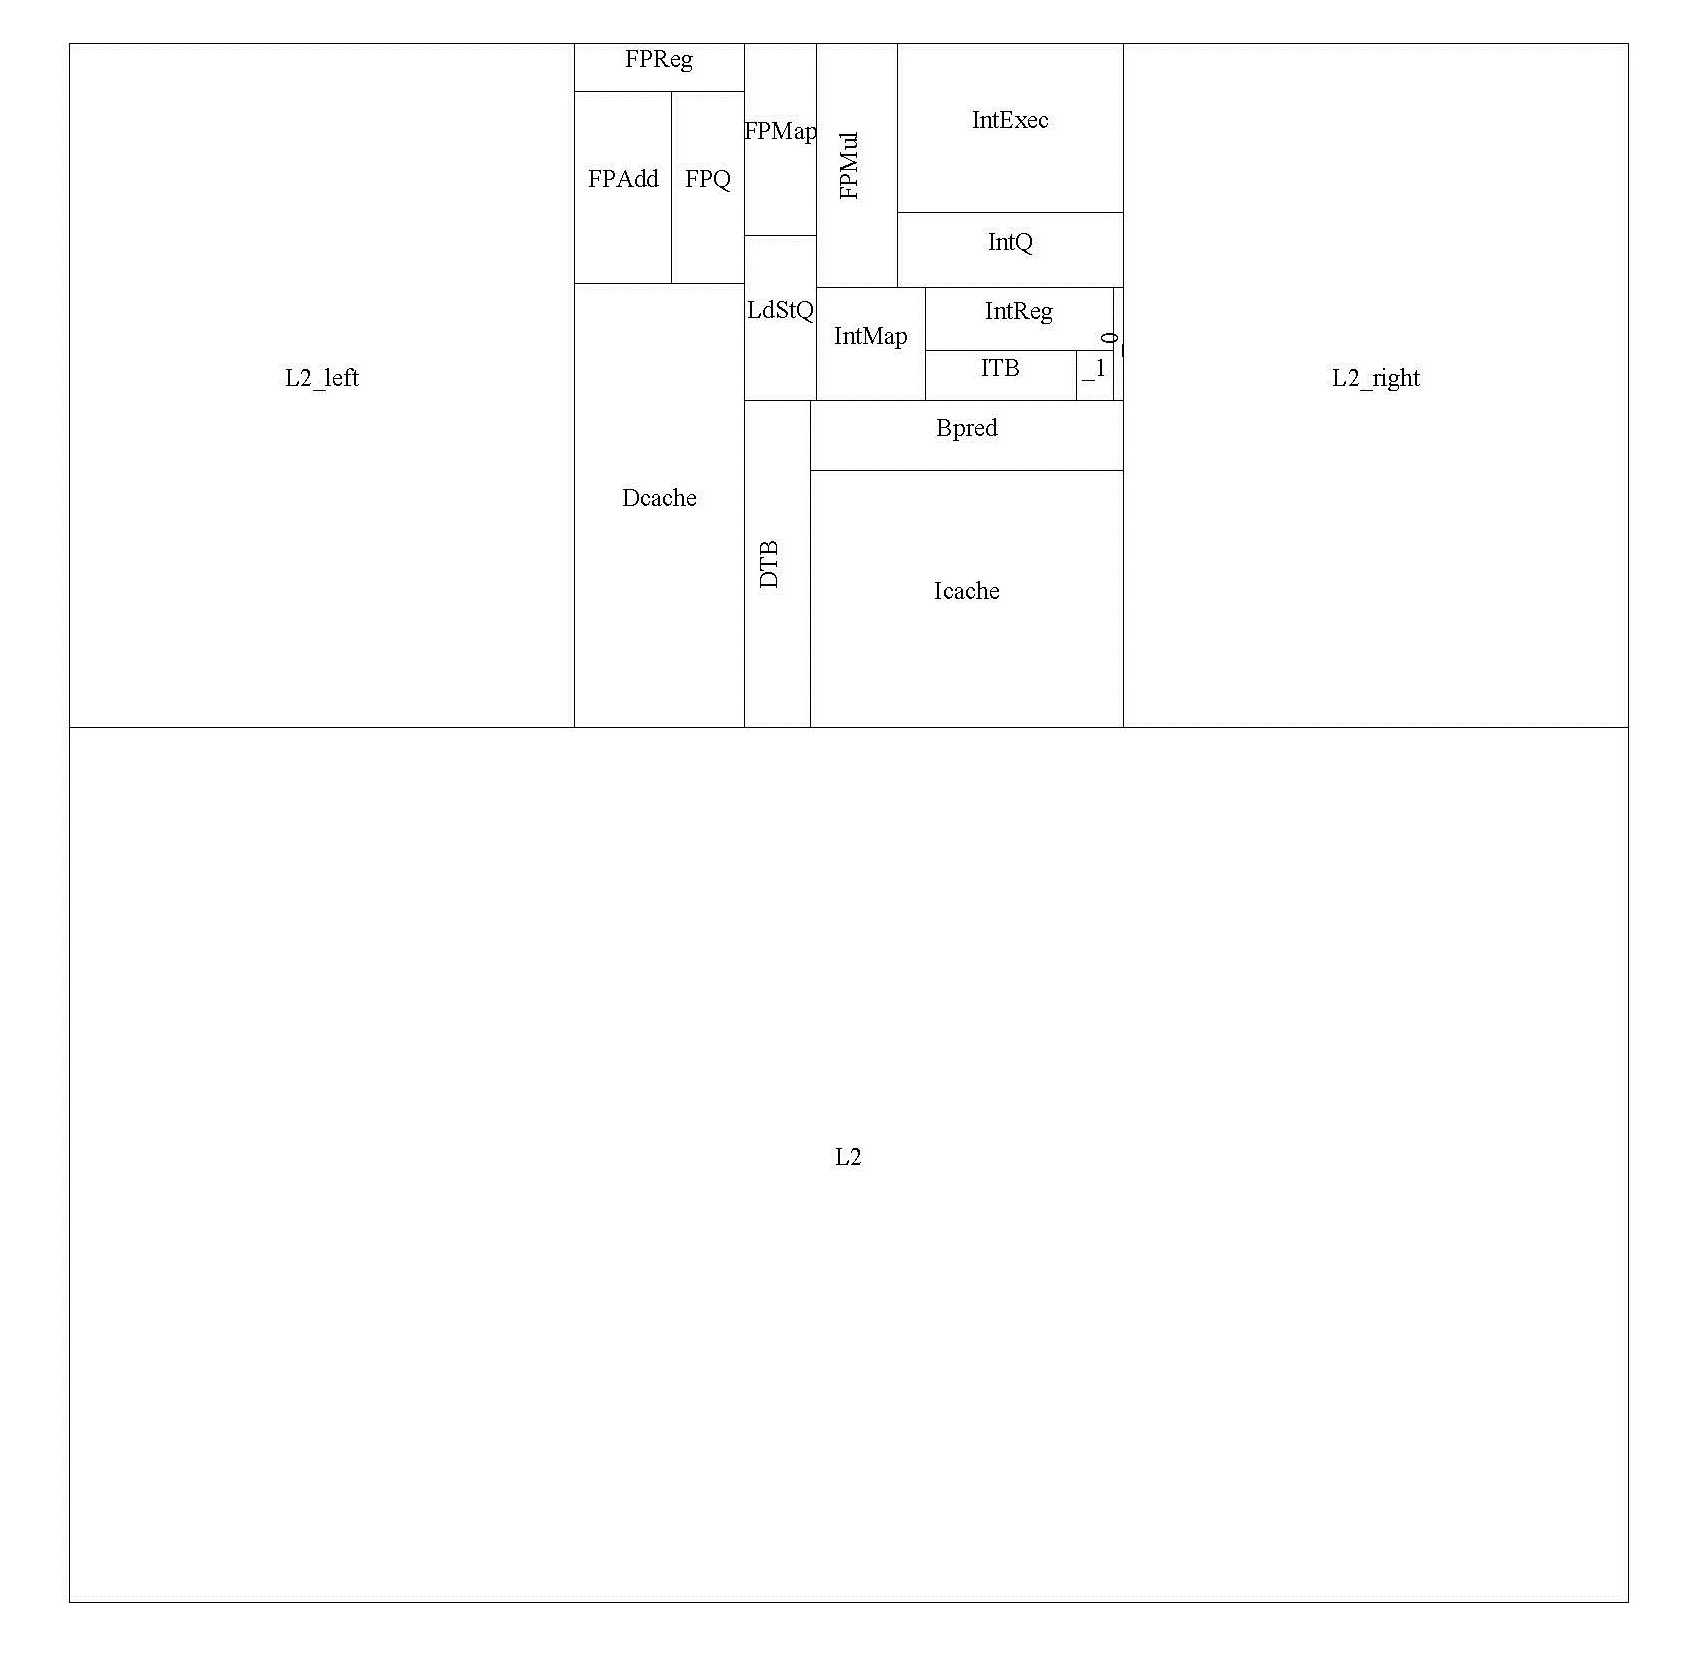
\includegraphics[width=1\textwidth,height=0.7\textheight]{EV6}
  \caption{Alpha21264芯片的物理布局}
  \label{fig:ev6}
\end{figure}


\subsection{芯片热分析及HotSpot模块级模型}

在MPSoC结构级热分析中,一般采用已有的电热等效模型,分析稳态温度分布,以降低计算复杂度[7,8]。 对于稳态热分析而言,将芯片的功耗分布作为注入的热流向量$\mathbf{P}$,对芯片的物理结构进行离散化建模后, 可以获得节点之间的热导矩阵$\mathbf{G}$, 目前多采用如下的稳态热分析方程计算节点温度分布向量$\mathbf{T}$:
\begin{equation}
\label{equ:chap4:gtp}
\mathbf{G} \times \mathbf{T} = \mathbf{P}
\end{equation}
对于多核实时功耗温度管理(dynamic power and temperature management, DPTM)研究\onlinecite{ThmBefMulCrFlrPlLimSty,TemSupVolPerfPowMdlMicroLvl}, 目前广泛采用Skadron等人提出的HotSpot热分析模型(软件)\onlinecite{TemMicroArch}构建热导矩阵$\mathbf{G}$, 并采用式\ref{equ:chap4:gtp}进行计算。 HotSpot采用基于等效热导的电路模型,将体系结构级的功能模块作为分析热点的对象。除了模块级别的热分析模型, HotSpot仍然提供了更为复杂的网格级(grid mode)热分析模型与方法。本文所指的HotSpot模型及其计算结果均指模块模式(block mode)的热分析模型与结果。 直观的对应芯片以及芯片热封装的物理构造的具体建模如图\ref{fig:hotspot-model} 所示。电路模型在垂直热传导方向上有3层:内核(die)层、扩热(heat spreader)层、与散热片(heatsink)层,另外加入第4层热对流(heat convector)层,即与环境温度的接口。内核层根据处理器的功能布局被分为对应的功能模块;扩热层分为5块: 与内核层完好对应的$R_sp$以及4块呈梯形状的环绕块;散热片层按照与扩热层相似的划分方法,分为$R_hs$以及4个环绕块; 最后,从热封装到外界环境的热对流层由$R_convection$表示\onlinecite{ThrOptTskAllocThemConstMulPro,MySSTAPaper}。 层与层之间模型刻画由内核直至封装及外界环境的热流; 层内水平模型刻画相邻模块间的热扩散。内核层产生的功耗等效为每个模块中心的电流源\onlinecite{TemMicArcMdlImpl,MySSTAPaper}。 用HotSpot计算分析Alpha 21264芯片的温度分布如图\ref{fig:ev6-grid-temp-surf}所示。

\begin{figure}[H]
  \centering
  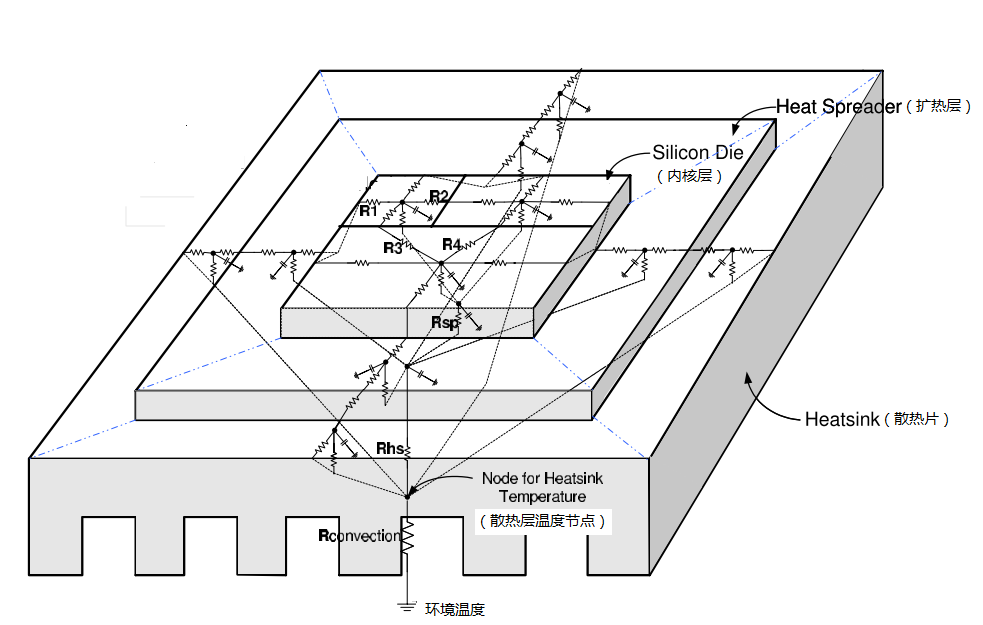
\includegraphics[width=1\textwidth,height=0.45\textheight]{HOTSPOT-MODEL}
  \caption{HotSpot对芯片的电路等效热分析模型}
  \label{fig:hotspot-model}
\end{figure}

\begin{figure}[H]
  \centering
  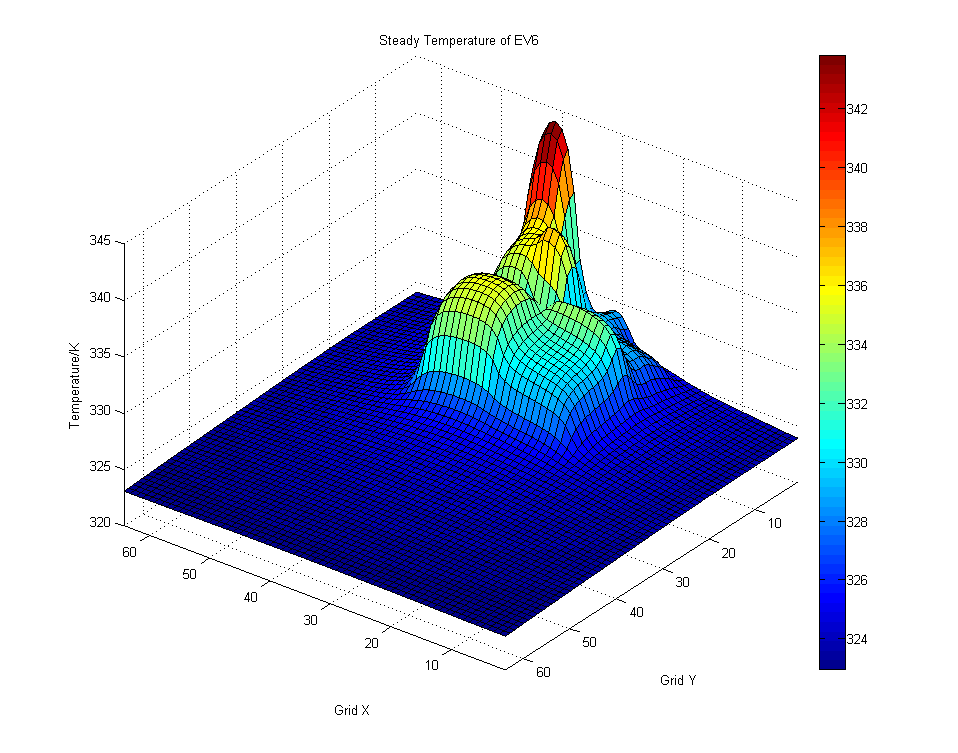
\includegraphics[width=1\textwidth,height=0.6\textheight]{EV6-GRID-TEM-SURF}
  \caption{Alpha21264芯片的温度分布}
  \label{fig:ev6-grid-temp-surf}
\end{figure}


\subsection{电热耦合效应:温度对漏电流功耗的影响}
正如\ref{sec:power}节中,式\ref{equ:chap2:active-power-simplified}、式\ref{equ:chap2:leakage-power} 所定性与定量地描述那样,芯片功耗由不仅包含运行功耗(动态功耗$P_{dynamic}$),还包括与热相关的静态功耗$P_{leakage}$。 近年来,芯片制作工艺的提高使得$P_{leakage}$已成为芯片功耗的主要贡献者。 而工作温度$T$的升高可以明显增大$P_{leakage}$。这就是所谓的芯片内部电热耦合效应。在考虑电热耦合效应的热分析过程中, 需要对$T-P$采用迭代方法计算,如\ref{fig:tp-iteration}所示, 对于一个16核CPU的测例(具体的实验参数设置见第\ref{cha:SSTAexperiments}章),对比了采用迭代算法和不采用迭代算法的分析结果。

与不考虑电热耦合效应的初始解相比,芯片峰值温度与静态功耗都有了明显的增加, 这表明在芯片的温度分析中、如果不考虑温度对静态功耗的影响,将会产生较大的分析误差。同时,与不考虑电热耦合效应的温度分析算法相比, 考虑电热耦合效应的温度分析算法需要经过7次迭代计算才能获得精确解, 换句话说,其算法复杂度将是对比算法的7倍。因此,出于热分析精度和热分析速度这两方面的考虑, 都应当降低考虑电热耦合效应的温度分析算法复杂度。
\begin{figure}[H]
  \centering
  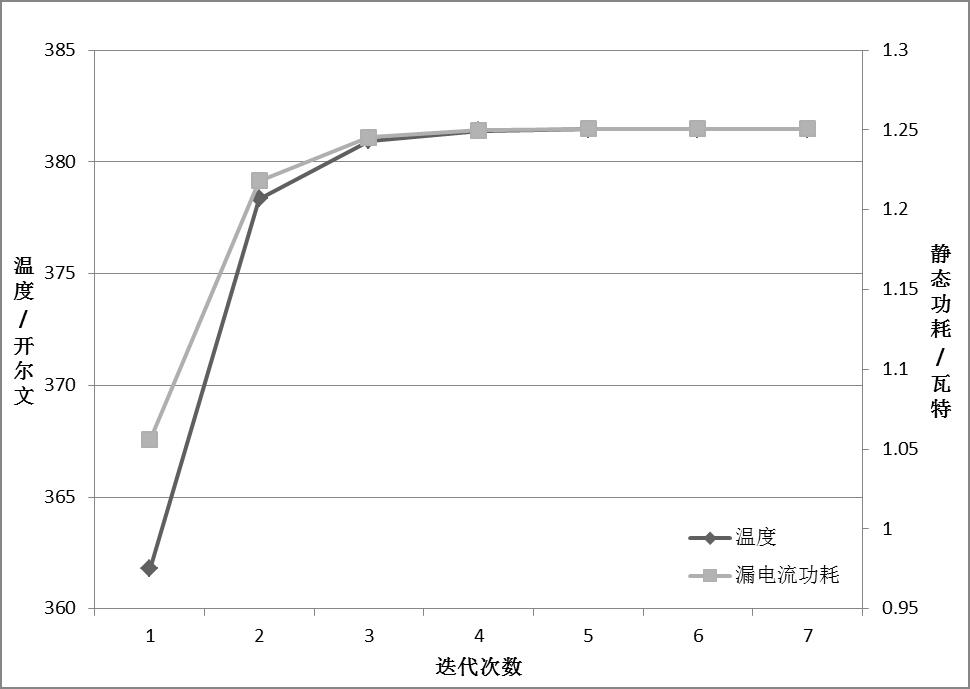
\includegraphics[width=1\textwidth,height=0.6\textheight]{TP-ITERATION}
  \caption{考虑电热耦合效应的多核芯片最高温度与静态功耗的迭代求解}
  \label{fig:tp-iteration}
\end{figure}


\section{3种MPSoC结构级热分析算法}
\label{sec:SSTAmethod}

\subsection{模块级热分析算法(简称BlockTAM算法)}
为了对功能模块进行热分析建模,按照式\ref{fig:hotspot-model}对HotSpot的多核芯片热分析模型, 采用等效电路的方法对其进行进一步简化, 为此本文假设\onlinecite{MySSTAPaper}:每个功能模块内的功耗与温度分布是均匀的,以该模块中心点的温度作为该模块的温度, 并将功耗密度乘以面积作为该模块的功耗,加于模块中心点。
在本文工作中,将模块$u$的功耗$P_{u,u}$作为注入热源。对于多核芯片, 如果仅在模块$u$加上幅值为$P_{u,u}$的阶跃激励, 其他模块均不加激励,则可以使用HotSpot模拟器获得所有模块的温度$T_{v,u}$响应曲线。 先根据$T_{u,u}$的最终收敛值$\overline{T}_{u,u}$ 可以计算出模块$u$的等效热阻$R_{u,u}$,计算公式为\ref{equ:chap4:blotam-rii}
\begin{equation}
\label{equ:chap4:blotam-rii}
R_{u,u} = \frac{\overline{T}_{u,u}}{P_{u,u}}
\end{equation}
再根据等效热阻$R_{u,u}$以及模块$v$功耗$P_{v,v}$的阶跃激励作为单一注入热源所得到的$\overline{T}_{u,v}$, 可以采用式\ref{equ:chap4:blotam-rij}计算出反映$P_{v,v}$对模块$u$温度作用关系的等效热阻$R_{u,v}$,
\begin{equation}
\label{equ:chap4:blotam-rij}
R_{u,v} = \frac{\overline{T}_{u,v}}{P_{v,v}}
\end{equation}
最后根据所获得的参数$R_{u,u}$与$R_{u,v}$ ,可以计算$P_{v,v}$对模块$u$温度计算产生影响的等效热源$P_{u,v}$:
\begin{equation}
\label{equ:chap4:blotam-pij}
P_{u,v} = \frac{\overline{T}_{u,v}}{\overline{T}_{u,u}}P_{u,u} = \frac{R_{u,v}\times P_{v,v}}{R_{u,u}\times P_{u,u}}P_{u,u}=\frac{R_{u,v}}{R_{u,u}}P_{v,v}
\end{equation}
因此,按照图\ref{fig:multicore-temp-model}中所给出的单模块温度分析模型,可以列出如下热分析表达式:
\begin{equation}
\label{equ:chap4:blotam-tii}
T_{u,u} = R_{u,u}\sum\limits_{v=1}^N P_{u,v} = R_{u,u}\widehat{P_{u}}
\end{equation}
其中$N$为多核芯片中的功能模块数目,$\widehat{P_{u}} = \sum\limits_{v=1}^N P_{u,v}$为模块$u$的等效热源,由于一个模块只有一个等效热源, 可见式\ref{equ:chap4:blotam-tii}提供的单模块热分析模型兼容了经典的单核(单模块)热分析模型\onlinecite{TemMicArcMdlImpl}。 从式\ref{equ:chap4:blotam-tii}可知:BlockTAM方法的算法时间复杂度与空间复杂度均为$O(N^2)$, 即算法复杂度为$O(N^2)$。
\begin{figure}[H]
  \centering
  
\includegraphics[width=1.0\textwidth,height=0.35\textheight]{MULTICORE-TEMP-MODEL}
  \caption{多核实时功耗温度管理的单模块与单核热分析简化等效电路模型}
  \label{fig:multicore-temp-model}
\end{figure}

\subsection{核级热分析方法(简称CoreTAM算法)}
为了对处理器核进行热分析建模,可以基于图\ref{fig:hotspot-model}中HotSpot的多核芯片热分析模型, 采用等效电路的方法对其进行进一步简化,为此,进行如下的假设\onlinecite{MySSTAPaper}:
\begin{enumerate}[1)]
\item 在处理器核多个功能模块中,逻辑模块(包括ALU等器件)产生最高的工作温度,将逻辑模块的温度作为处理器核的温度; 为了对其他核产生影响,逻辑模块中心被注入处理器核中对应功能模块的功耗。
\item 为了计算温度对漏电流功耗的影响,将逻辑模块的静-动态功耗比例、作为处理器核中所有功能模块的静-动态功耗比例。
\end{enumerate}

基于如上假设,将核p内的所有模块均加上符合核内功耗比例要求的阶跃激励,其他核均不加激励, 则可以使用HotSpot模拟器获得所有核的温度$T_{t,s}$响应曲线。先根据$T_{s,s}$的最终收敛值$\overline{T}_{s,s}$ 可以计算出核$s$的等效热阻$R_{s,s}$,计算公式如下:
\begin{equation}
\label{equ:chap4:cortam-rpp}
R_{s,s} = \frac{\overline{T}_{s,s}}{P_{s,s}}
\end{equation}
式\ref{equ:chap4:cortam-rpp}中$P_{s,s}$是核$s$内所有模块的功耗之和。再根据等效热阻$R_{s,s}$, 以及核$t$功耗$P_{t,t}$ 的阶跃激励作为单一注入热源所得到的$\overline{T}_{s,t}$,采用如下公式计算出反映$P_{t,t}$对核$s$ 温度作用关系的等效热阻$R_{s,t}$,
\begin{equation}
\label{equ:chap4:cortam-rpq}
R_{s,t} = \frac{\overline{T}_{s,t}}{P_{t,t}}
\end{equation}
之后根据以上所获得的参数,可以计算$P_{t,t}$对核$s$温度计算产生影响的等效热源$P_{s,t}$:
\begin{equation}
\label{equ:chap4:cortam-ppq}
P_{s,t} = \frac{\overline{T}_{s,t}}{\overline{T}_{s,s}}P_{s,s} = \frac{R_{s,t}\times P_{t,t}}{R_{s,s}\times P_{s,s}}P_{s,s} = \frac{R_{s,t}}{R_{s,s}}P_{t,t}
\end{equation}
最后,按照图\ref{fig:multicore-temp-model}中所给出的热分析模型,可以列出如下热分析表达式:
\begin{equation}
\label{equ:chap4:cortam-tpp}
T_{s,s} = R_{s,s}\sum\limits_{t=1}^n P_{s,t}
\end{equation}

式\ref{equ:chap4:cortam-tpp}中$n$为多核芯片中的核数。从式\ref{equ:chap4:cortam-tpp}可知: CoreTAM方法的算法复杂度为$O(n^2)$。 从计算机系统结构可知, 核数$n$远小于模块数$N$,因此,多核芯片的核级温度分析复杂度要远小于模块级。

\subsection{考虑核内模块相互影响的改良核级热分析方法(简称BlockInsideCoreTAM算法)}
在核级热分析方法研究中,假设了核内各个模块对核内逻辑模块中心温度具有相同的相关热阻, 并且每个核内仅需计算一个点的温度;核内各模块均使用该温度来刷新模块的漏电流功耗, 会使整个核的漏电流功耗增大。为了使漏电流计算更为精确,必须计算出各自模块的温度,为此, 下面给出一个考虑核内模块相互影响的改良核级热分析方法:BlockInsideCoreTAM。在BlockInsideCoreTAM方法中, 先进行如下的假设\onlinecite{MySSTAPaper}:
\begin{enumerate}[1)]
\item 核$t$的功耗$P_{t,t}$对核$s$内所有模块均产生相同的等效热量影响为$P_{s,t} = \frac{R_{s,t}}{R_{s,s}}P_{t,t}$,其中$R_{s,t}$为两个核内所有模块之间相关热阻的平均值,即
\begin{equation}
\label{equ:chap4:bicortam-rpq}
R_{s,t} = \frac{1}{m^2}\sum\limits_{u \in BS_s}\sum\limits_{v \in BS_t}R_{u,v}
\end{equation}
式\ref{equ:chap4:bicortam-rpq}中$BS_x$是核$x$内所有模块的集合。
\item 在核$s$内,模块$v$对模块$u$的等效热量影响为$P_{u,v} = \frac{R_{u,v}}{R_{u,u}}P_{v,v}$,式中$u,v \in BS_s$。
\end{enumerate}
按照以上假设,可以列出如下BlockInsideCoreTAM表达式:
\begin{equation}
\label{equ:chap4:bicortam-tii}
\frac{T_{u,u}}{R_{u,u}} = \sum\limits_{t=1,t\neq s}^n P_{s,t} + \sum\limits_{v=1}^m P_{u,v}
\end{equation}
从式\ref{equ:chap4:bicortam-tii}可知:BlockInsideCoreTAM方法的算法复杂度为$O(n^2+(m^2-1)n)$。 BlockInsideCoreTAM的计算复杂度介于CoreTAM和BlockTAM之间,当$m \ll n$时,BlockInsideCoreTAM的算法复杂度近似等于CoreTAM。

